\chapter{Моделирование работы искусственного сердечного клапана} \label{chapt3}

Как отмечалось ранее, искусственные сердечные клапаны являются одними из самых
сложных биопротезов, используемых в кардиохирургии. Они достаточно эффективно
позволяют бороться с заболеваниями и повреждениями естественных клапанов, но
при этом не являются достаточно долговечными и при их использовании могут
проявляться побочные явления. Например, механические клапаны обладают высокой
надежностью и долговечностью, но могут приводить к сильным деформациям потока,
формированию сгустков кровяных клеток и как следствие - к образованию тромбов.
Биологические клапаны лишены этого недостатка, однако они менее долговечны и их
изготовление достаточно сложная техническая задача, которая до сих пор
полностью не решена.

Данная глава посвящена результатам применения модели, описанной в главе \ref{chapt1},
для моделирования работы искусственного трехстворчатого клапана. Клапан расположен в
сосуде произвольной формы, закреплен фиброзным кольцом на его стенках, и приводится
в движение посредством перепада давления неоднородной несжимаемой жидкости в сосуде.
Эта модель применима, например, к аортальному клапану, который располагается на
границе левого желудочка и аорты, препятствуя обратному току крови из аорты в
левый желудочек на этапе диастолы.

Входными параметрами для данных расчетов являются:
\begin{itemize}
    \item Начальная форма клапана $\Gamma_4$ и сосуда $\Gamma_1$
    \item Жесткость клапана в каждой точке (коэффициенты $k_b$, $k_s$)
    \item Векторное поле скорости жидкости в начальный момент времени $\vec{u_0}$
    \item Распределение примеси в начальный момент времени
            (а соответственно, и концентрации $c_0$, вязкости $\mu_0$ и плотности $\rho_0$)
    \item Перепад давления $p_{in}$, $p_{out}$
\end{itemize}

В качестве результата моделирования мы получаем описание состояния системы
<<клапан-жидкость>> в каждый момент времени, т.е.:
\begin{itemize}
    \item Векторно поле скорости жидкости $\vec{u}$
    \item Скалярное поле давления жидкости $\vec{p}$
    \item Распределение примеси
    \item Текущая форма клапана
    \item Векторное поле напряжения деформации на поверхности клапана $F$
    \item Расход жидкости сквозь клапан
\end{itemize}

\section{Моделирование работы симметричного клапана} \label{sect3_1}

Одна из причин, по которой трехстворчатый сердечный клапан является крайне сложным
объектом для исследования, заключается в его сложной геометрии. Для каждого человека
она в той или иной степени уникальна, т.к. присутствуют отклонения от стандартной
формы. На первом этапе мы опустим эти сложности и будем рассматривать клапан идеальной
формы с тремя симметричными створками. Его схема изображена на рис. \ref{img:symmetric_valve}

\begin{figure}[ht]
  \center
  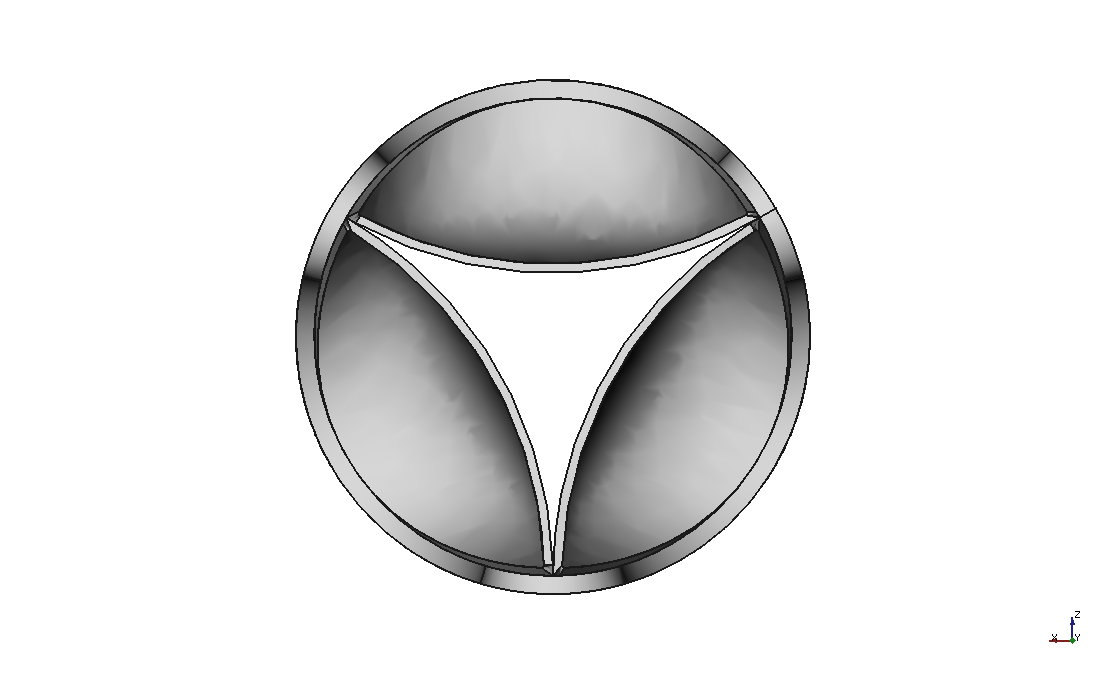
\includegraphics [scale=0.27] {SymmetricValveFront.png}
  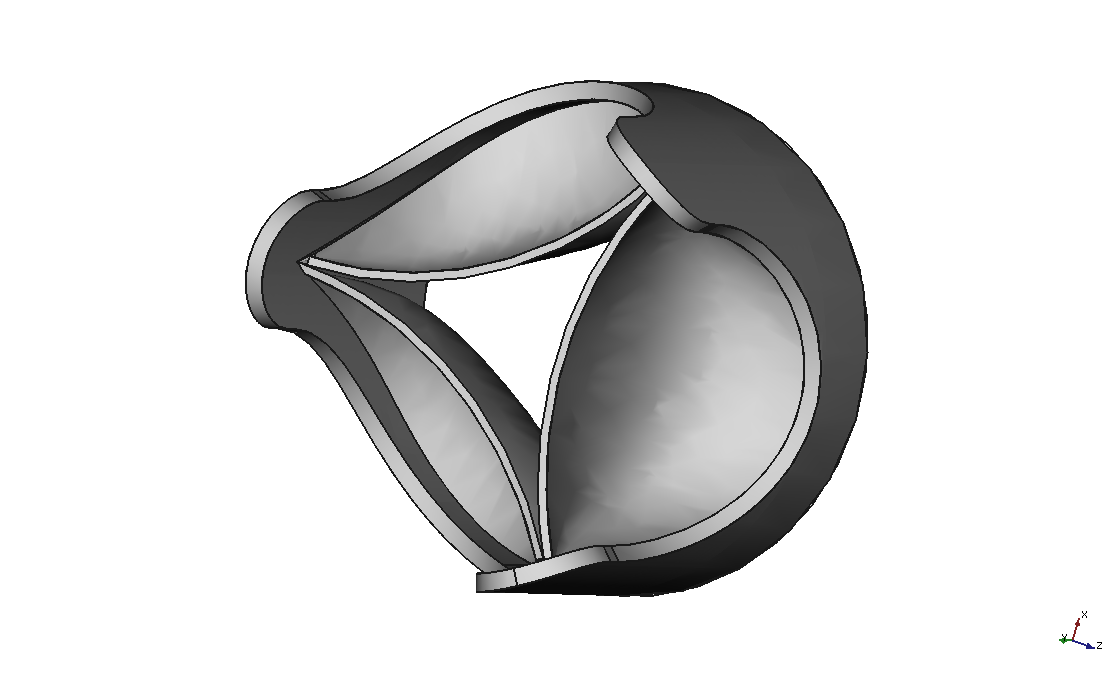
\includegraphics [scale=0.27] {SymmetricValveSide.png}
  \caption{Клапан идеальной формы с тремя симметричными створками}
  \label{img:symmetric_valve}
\end{figure}

Т.к. фиброзное кольцо в данном случае полностью совпадает с поверхностью сосуда,
в котором находится клапан, и стенки сосуда являются твердыми, мы можем его убрать,
переместив всю жесткость кольца на линию, по которой лепестки клапана соединяются
со стенками сосуда. Итоговая схема расчета изображена на рис. \ref{img:aorta_valve_scheme_flat}

\begin{figure}[ht]
  \center
  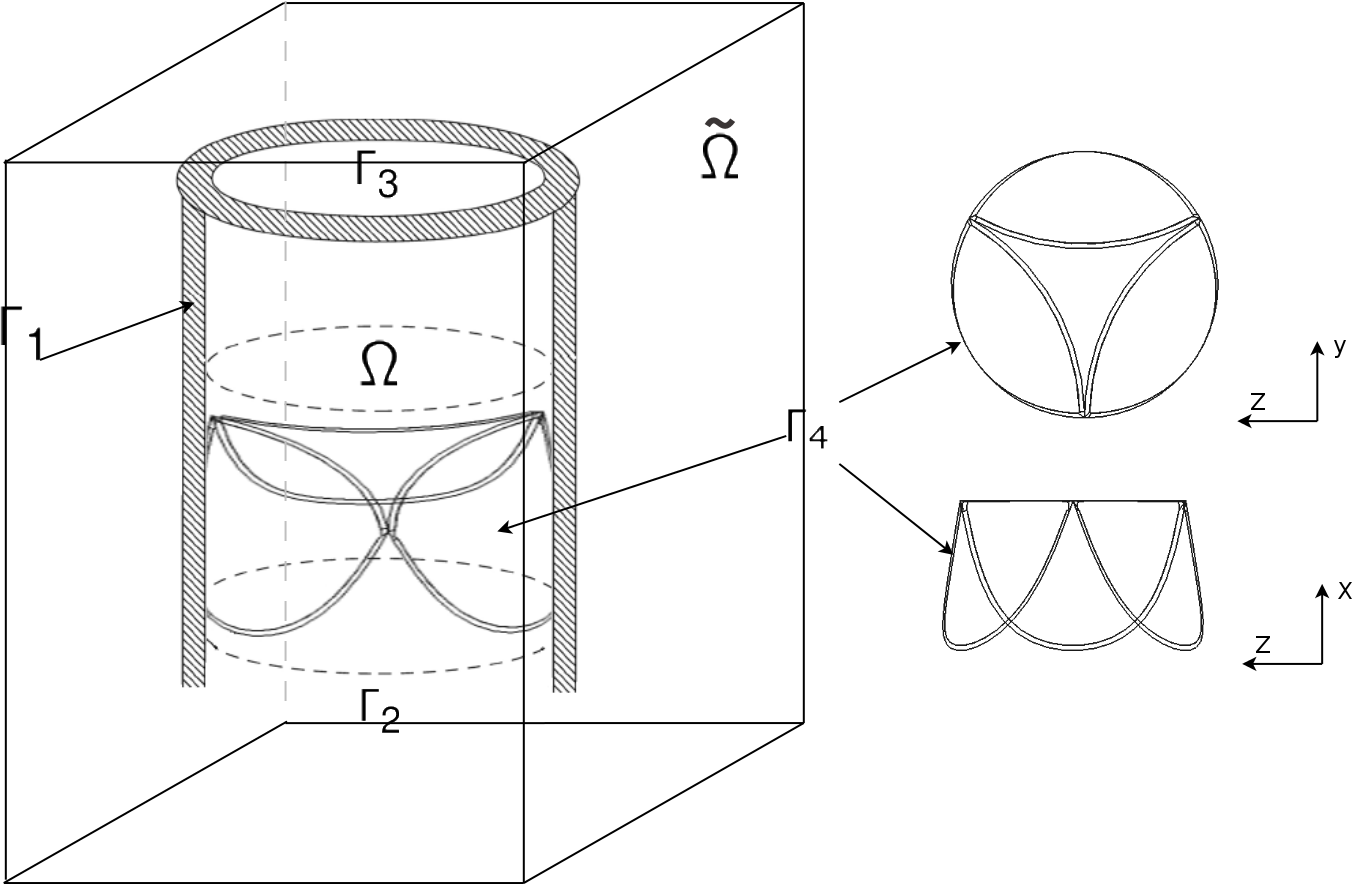
\includegraphics [scale=0.27] {aorta_valve_scheme_flat_computation.png}
  \caption{Схема расположения клапана в сосуде}
  \label{img:aorta_valve_scheme_flat}
\end{figure}

Все описанные ниже расчеты проводились в безразмерных переменных.  В качестве
сосуда, в котором расположен клапан, используется круговой цилиндр длинной $l=1$,
радиусом $r=0.11$. Для стенок сосуда используется <<простая>> формула расчета
напряжения (\ref{eq:simple_force}) с коэффициентом жесткости $k=1 \cdot 10^{3}$.
Область $\tilde{\Omega}$ имеет размеры $10 \times 0.5 \times 0.5$.

При проектировании искусственных сердечных клапанов одним из самых главных его свойств
является полнота закрытия створок в момент диастолы, т.к. это основная функция
створчатого аппарата. Ниже на рис. \ref{img:valve_delaunay_with_markers}
приведены результаты моделирования одного цикла работы клапана
при периодически меняющемся от $0$ до $6$ перепаде давления $p_{in} - p_{out}$,
параболической зависимостью от времени на каждом периоде.
Для створок клапана заданы коэффициенты сопротивления растяжению $k_s = 5 \cdot 10^{3}$ и скручиванию
$k_b = 2 \cdot 10^{3}$. Внутри сосуда течет вязкая однородная несжимаемая жидкость $\rho=1$, $\mu=1\cdot10^{-2}$.
Для расчета задавалась конечно-разностная сетка $\tilde{\Omega_h}$, соответствующая области течения,
и неструктурированная сетка $\tilde{\Gamma_h}$, соответствующая стенками сосуда и створкам клапана.
Расстояние между узлами $\tilde{\Omega_h}$ $h_x = h_y = h_z = 0.01$. Сетка $\tilde{\Gamma_h}$
была получена путем конвертирования CAD модели идеального клапана в сеточный формат с расстояниями
между узлами меньше соответствующих $h_x, h_y, h_z$. Для рассчета был выбран шаг по времени $\triangle t = 0.01$.

\begin{figure}[ht]
  \center

  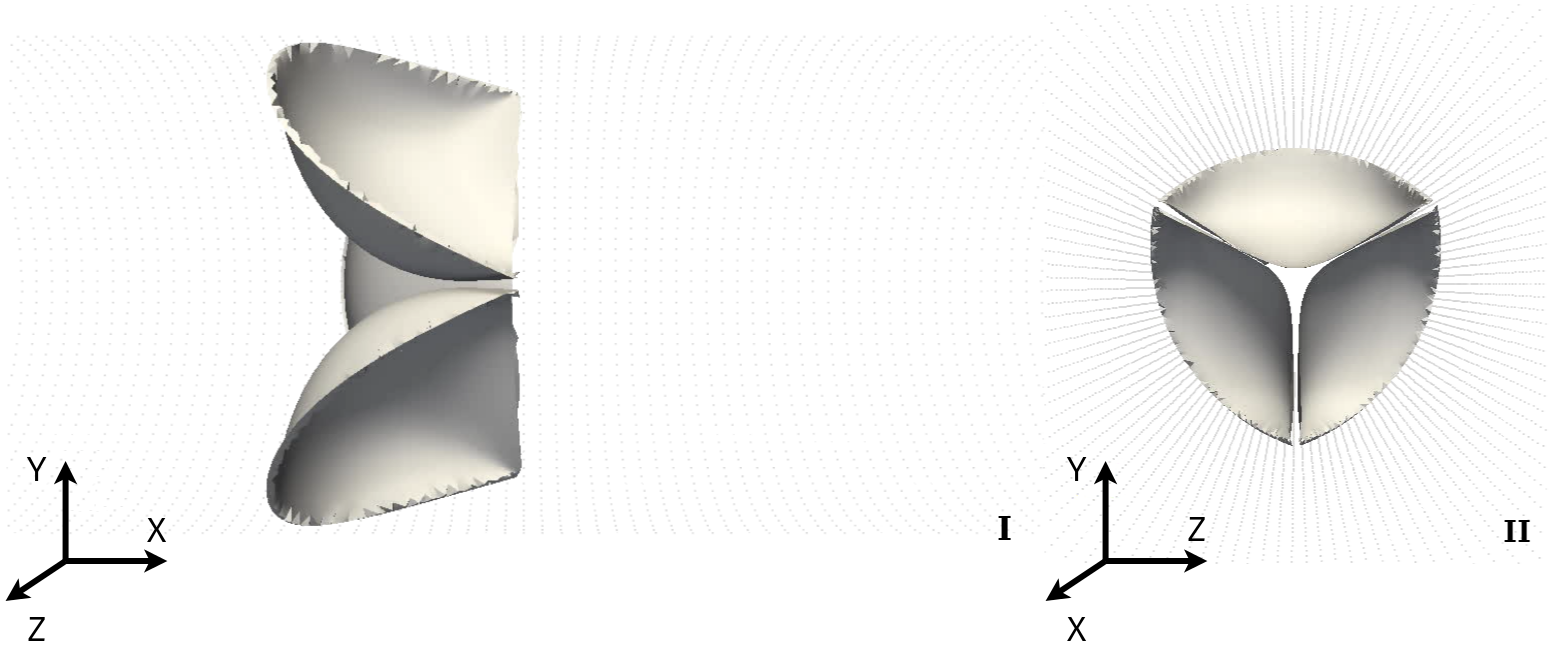
\includegraphics [scale=0.27] {valve_delaunay_with_markers1_axes.png}

  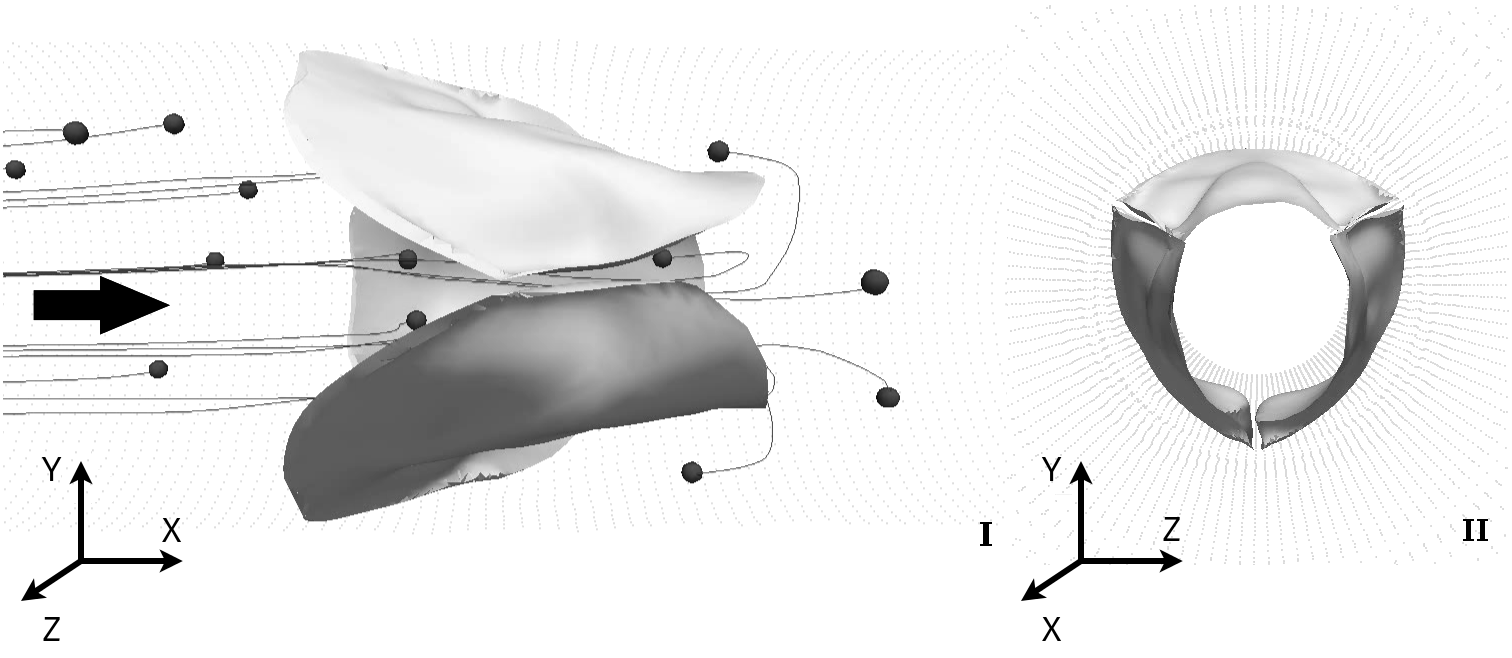
\includegraphics [scale=0.27] {valve_delaunay_with_markers2_axes.png}

  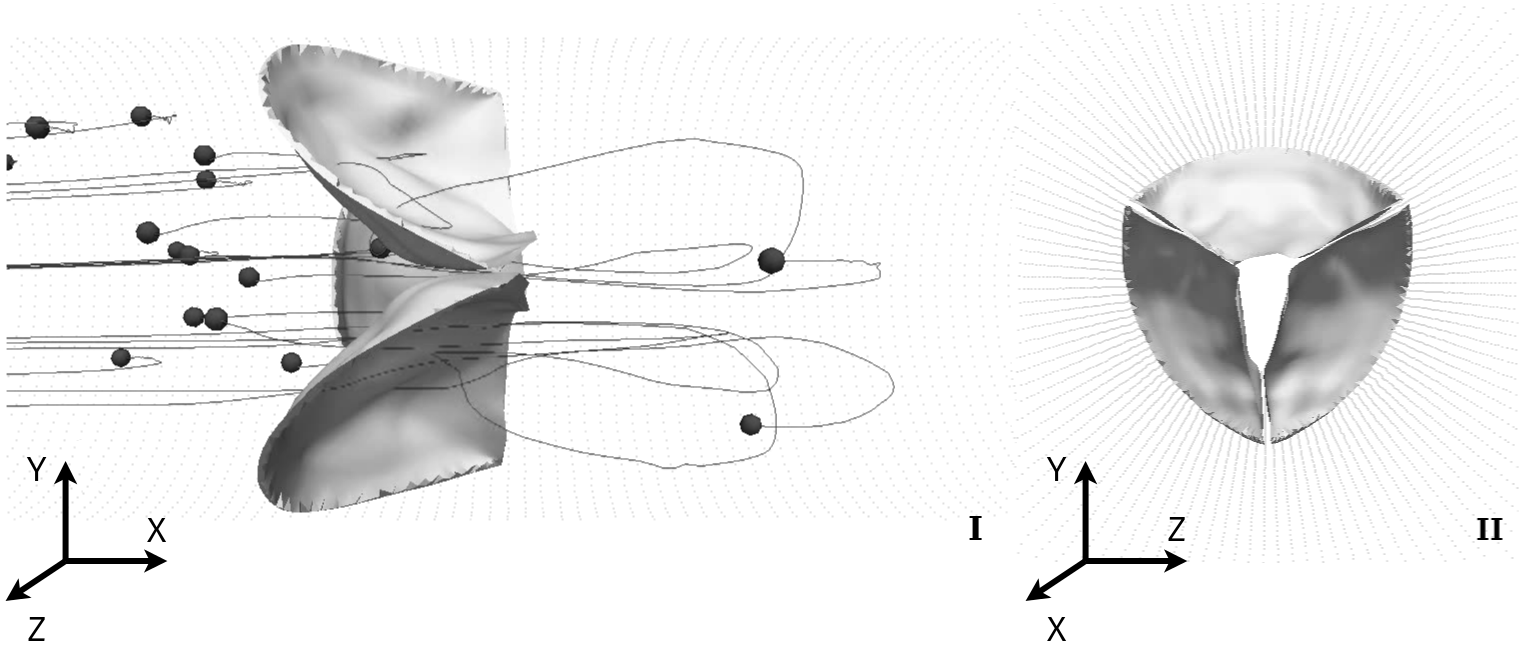
\includegraphics [scale=0.27] {valve_delaunay_with_markers3_axes.png}

  \caption{Динамика створок клапана и треки некоторых частиц. Направление тока
    указано стрелкой. Показан вид сбоку (I) и вид спереди (II) a) $t=0$, b)
    $t=0.7$, c) $t=1.5$}

  \label{img:valve_delaunay_with_markers}
\end{figure}

Этот расчет демонстрирует динамику формы створок клапана, а также треки частиц
жидкости, протекающей сквозь него. Створки клапана раскрываются при изменении
разности давлений, а затем возвращаются в исходное положение при выравнивании
давлений. В процессе движения створок возникают вихревые движения жидкости, при
закрытии часть жидкости успевает проникнуть назад через клапан до его закрытия
(так называемый, <<объем регургитации>>). В силу изначальной геометрии клапана
его закрытие происходит не полностью, т.к. перепад давления сильно отличается
от реалистичного, а также стенки сосуда являются абсолютно ровными, тогда как
в настоящих биологических системах на плотность закрытия клапана влияет наличие,
например, синусов Вальсальвы, которые деформируют течение.

Как было сказано ранее, во многих работах недостаточно акцентируется внимание
на влиянии течения жидкости на итоговое состояние системы. И одним из важных
аспектов нашей работы являются результаты моделирования работы трехстворчатого
клапана с учетом неоднородной структуры жидкости, протекающей сквозь него.

На рис. \ref{img:concentration_dynamics} показано изменение концентрации
форменных элементов при прохождении потока жидкости через клапан.
Большинство параметров для этого расчета аналогичны предыдущему,
за исключением того, что в сосуде течет неоднородная двухкомпонентная жидкость.
В начальный момент времени концентрация примеси в каждой точке равна
$c_0=0.45$, на входе задается постоянный приток примеси $c_s|_{\Gamma_2} = 0.45$.

\begin{figure}[ht]
  \center

  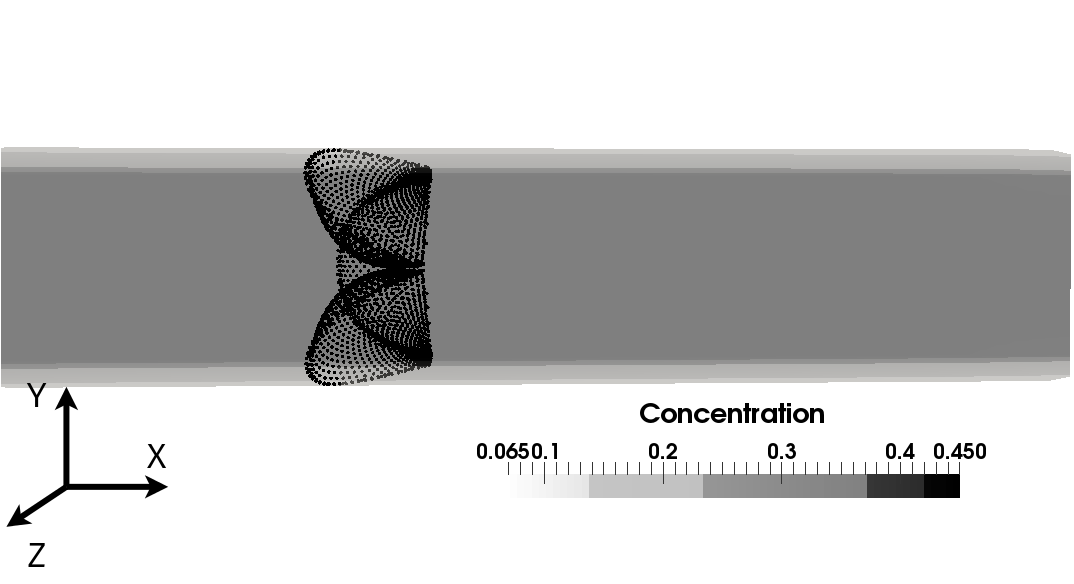
\includegraphics [scale=0.27] {concentration_1_axes.png}

  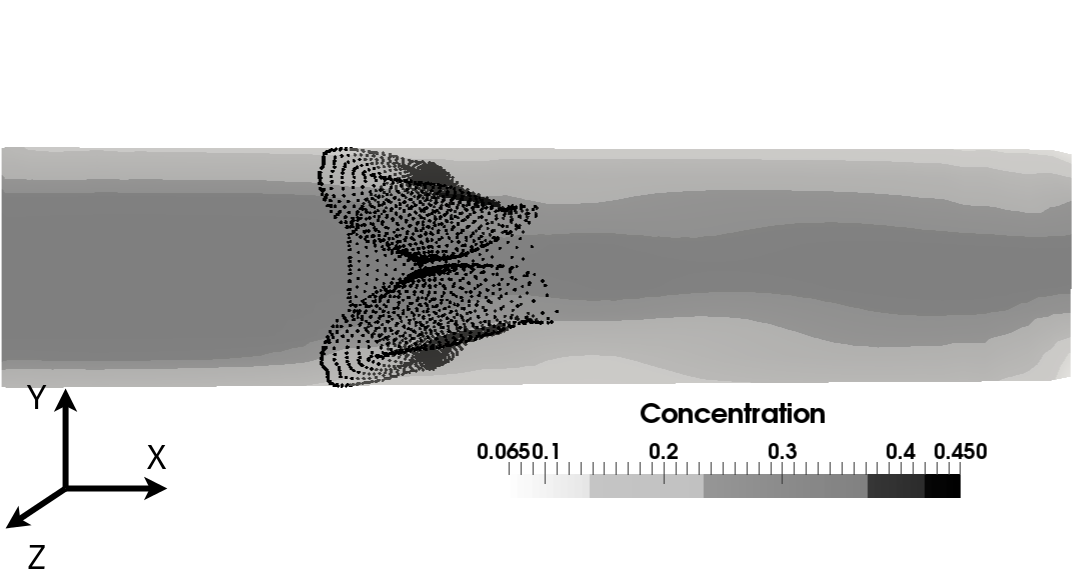
\includegraphics [scale=0.27] {concentration_2_axes.png}

  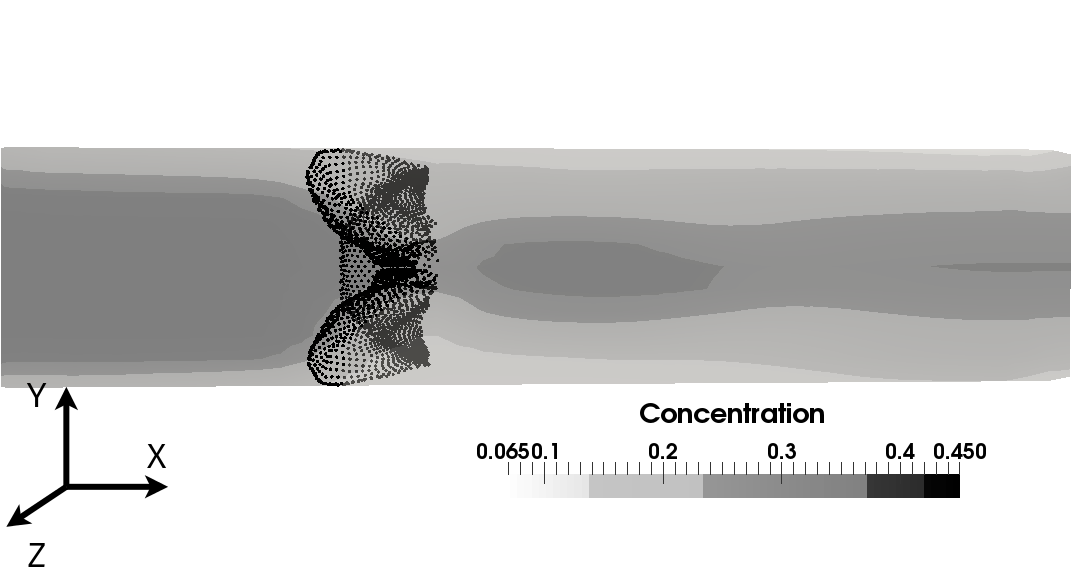
\includegraphics [scale=0.27] {concentration_3_axes.png}

  \caption{Движение створок клапана в сосуде с переменной вязкостью и плотностью.
    На входе задается постоянный приток примеси $c_s|_{\Gamma_2} = 0.45$,
    концентрация примеси в начальный момент времени $c_0=0.45$, $\rho_1=1,
    \rho_2=1.2, \mu_1=1 \cdot 10^{-2}, \mu_2=1.2 \cdot 10^{-2}$; a) $t=0$, b) $t=3$, c) $t=6$}

\label{img:concentration_dynamics}
\end{figure}

Финальное распределение показано после трех циклов работы клапана. Изначально
равномерное распределение форменных элементов со временем нарушается движением
створок клапана, приобретая пульсовый характер. Т.к. сам клапан не симметричен
по осям $Ox, Oy, Oz$, распределение примеси также не симметрично.

Но помимо неоднородной структуры жидкости крайне важным является итоговое
распределение напряжения деформации по поверхности створок клапана в разные
моменты времени, т.к. напряжение непосредственно влияет на его износ. Ниже
на рис. \ref{img:valve_stress_distribution} приведена динамика движения одной
из трех створок потоке неоднородной двухкомпонентной жидкости, а также визуализация
возникающего на ней напряжения.

\begin{figure}[ht]
  \center

  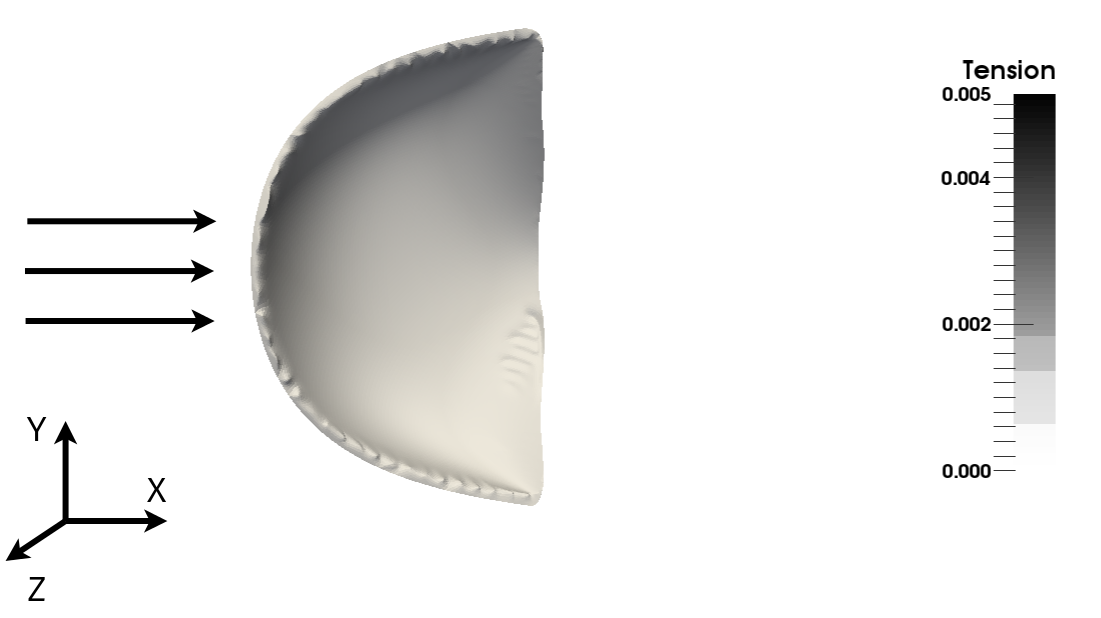
\includegraphics [scale=0.27] {ideal_valve_stress_1_better_axes.png}

  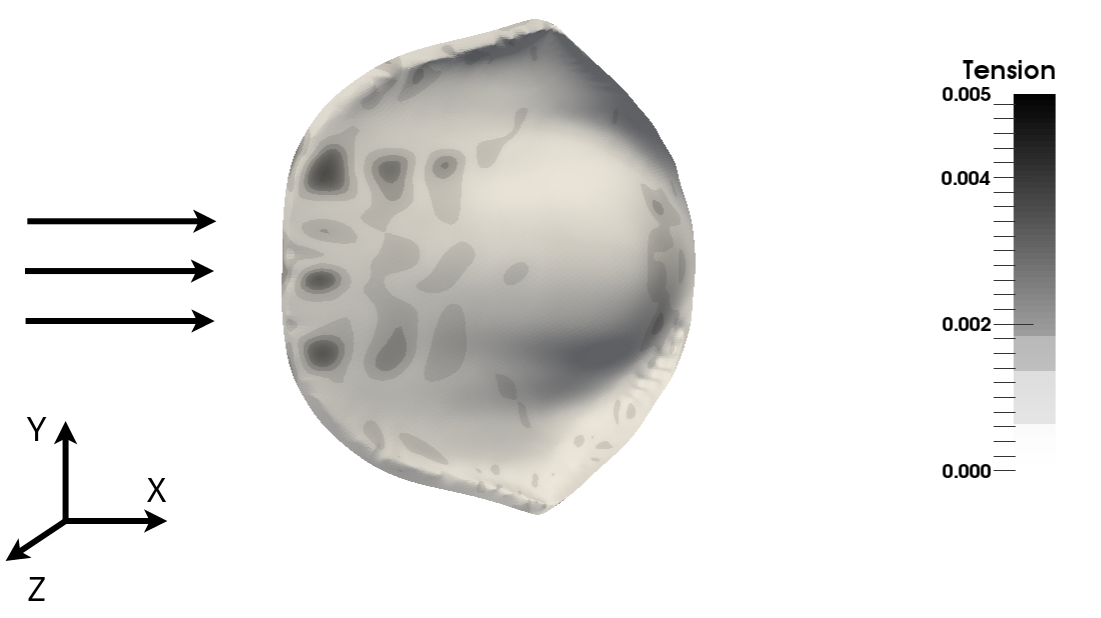
\includegraphics [scale=0.27] {ideal_valve_stress_2_better_axes.png}

  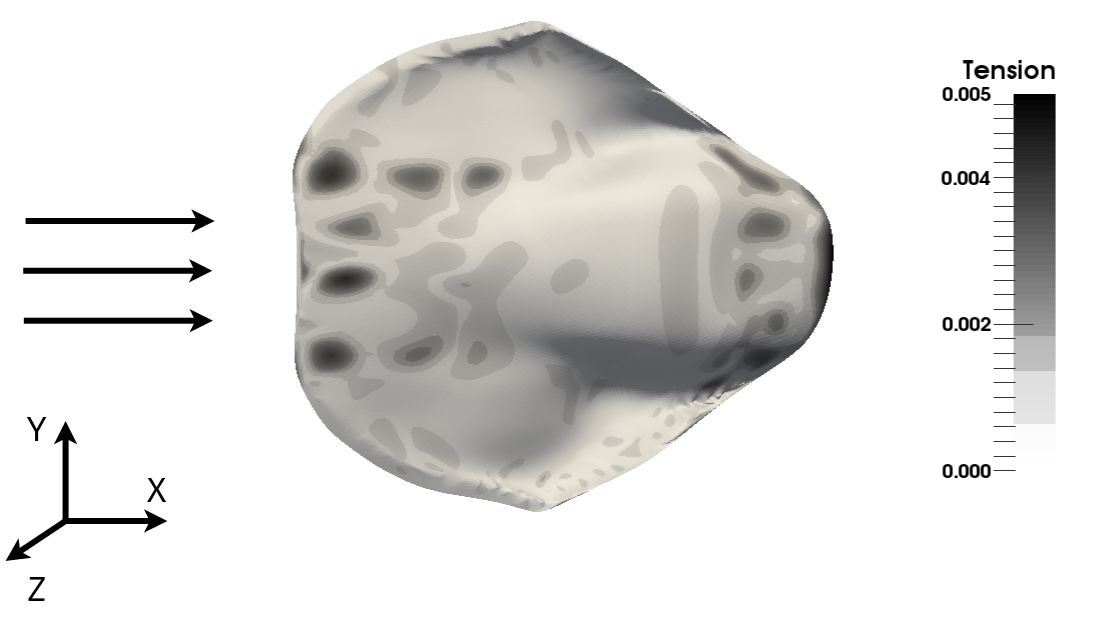
\includegraphics [scale=0.27] {ideal_valve_stress_3_better_axes.png}

  \caption{Распределение напряжение по поверхности створки в моменты времени $t=0,
    t=0.4, t=0.8$. Точками обозначены стенки сосуда}

\label{img:valve_stress_distribution}
\end{figure}


\section{Моделирование работы клапана <<Юнилайн>>} \label{sect3_2}

\section{Верификация модели} \label{sect3_3}

\clearpage
